\documentclass[conference]{IEEEtran}
\IEEEoverridecommandlockouts
% The preceding line is only needed to identify funding in the first footnote. If that is unneeded, please comment it out.
\usepackage{cite}
\usepackage{url}
\usepackage[english]{babel}
\usepackage{amsmath,amssymb,amsfonts}
\usepackage{algorithmic}
\usepackage{graphicx}
\graphicspath{ {./images/} }
\usepackage{textcomp}
\usepackage{xcolor}
\def\BibTeX{{\rm B\kern-.05em{\sc i\kern-.025em b}\kern-.08em
    T\kern-.1667em\lower.7ex\hbox{E}\kern-.125emX}}
\begin{document}

\title{Assignment for the course \\Automated Planning Theory and Practice\\
% {\footnotesize \textsuperscript{*}Note: Sub-titles are not captured in Xplore and
% should not be used}
% \thanks{Identify applicable funding agency here. If none, delete this.}
}

\author{\IEEEauthorblockN{Davide Lusuardi}
\IEEEauthorblockA{\textit{Department of information engineering and computer science} \\
\textit{University of Trento}\\
Trento, Italy \\
davide.lusuardi@studenti.unitn.it}
}

\maketitle

\begin{abstract}
This report is intended to present and analyze the assignment for the course 
\textit{Automated Planning Theory and Practice} \ref{TODO:assignment_document}
and discuss some design choices regarding its modeling and implementation.

The assignment is inspired by an emergency services logistics scenario where
a set of robotic agents have the task to deliver crates containing emergency 
supplies to some injured people.

The assignment is divided into four subproblems, each building on the previous 
one with increasing complexity.
In the first problem, the robot can pick up and move just one crate at time.
In the second problem, the complexity increase a bit given that the robot
exploits a carrier that can load up to four crates.
In the third problem, is required to use durative actions in order to assign
reasonable duration to different actions and model which actions can be executed
in parallel.
Lastly, the third problem has to be implemented within the \texttt{PlanSys2} 
framework, executing in a simulated environment the plan.


% This report is intended to present and discuss some design choices regarding 
% the modeling and implementation of the scenario and the four subproblems 
% proposed in the assignment document \ref{TODO}.
% In this paper, we present and discuss some methods for free-viewpoint synthesis for soccer games.
% These techniques permit to generate novel views of actions from any angle and allow viewers to virtually fly through real soccer scenes.

% In this document, we discuss some methods to accomplish free-viewpoint video visualization for soccer scenes.
% These methods generate novel views of actions from any angle and allow viewers to virtually fly through real soccer scenes.
% TODO: complete
% and is of interest for visualization in TV productions.
\end{abstract}

% \begin{IEEEkeywords}
% component, formatting, style, styling, insert
% \end{IEEEkeywords}

\section{Introduction}
Planning is a branch of Artificial Intelligence that seeks to automate reasoning about
formulating a plan to achieve a given goal in a given situation. 
Planning is a model-based approach: a planning system takes as input a model of the initial state, 
the actions available to change it and the goal conditions, producing as output a plan 
that will reach the goal from the initial situation.

The Planning Domain Definition Language (PDDL) is a formal knowledge representation language 
designed to express planning models. Developed by the planning research community, 
it has become a de-facto standard language of many planning systems.

The purpose of the assignment is two-fold: first, to model the given scenario using the PDDL language 
and find a plan using a state-of-the-art planner; second, leveraging the \texttt{PlanSys2} \cite{PlanSys2} 
infrastructure, to integrate the model within a robotic setting.

ROS2 Planning System, \texttt{PlanSys2} in short, is a framework for symbolic planning that incorporates 
novel approaches for execution on robots working in demanding environments \cite{PlanSys2}.

The proposed scenario is inspired by an emergency services logistic problem:
a number of injured people are situated at known locations and one or more robotic agents
have the task to deliver crates containing emergency supplies to each person. 
The planning system should formulate a plan for the robotic agents in order to deliver all
the crates needed by the injured people.

The document is structured as follows: in Section \ref{sec2},
we explain in details our understanding of the proposed scenario and the four subproblems; 
in Section \ref{sec3}, we describe the design choices and the proposed solutions to solve the problem,
making some assumptions in order to constrain the problem; % TODO: scrivere meglio
in Section \ref{sec4}, we discuss and analyze the achieved results and briefly describe the
content of the submitted archive; in Section \ref{sec5}, we make some conclusions and future 
works are proposed.




\section{Understanding of the problem}
\label{sec2}

The assignment proposes four subproblems within the same scenario, each building on the previous one.

The proposed scenario consists of an emergency situation in which there are a number of injured people 
who need emergency supplies.
% to help delivering them some crates containing
Each injured person is located in a specific place and may need some kinds of emergency supply
(e.g. food, medicine, beverage, ...). There may be more people at the same location and some 
locations may be empty.
Each crate is at a specific location and contains just one specific kind of emergency supply.
Some people may already have some crates and some others may not need any crate.
People don't care which crate exactly they get, only the content type is important.
There can be one or more robotic agents that cooperate in order to deliver crates to people.
Each location is connected to every other location, so the robotic agent can move directly between them.
Initially, the robotic agents and the crates are situated at the depot, where there are not injured people.

The goal consists in deliver all the required crates to injured people.

The above considerations and the goal are common for all the four subproblems that we are going to discuss.

\subsection{Problem 1}
This is the easiest problem.
We have that a single robotic agent is present at the depot.
It can perform the following actions: pick up and load just one crate that is at the same location;
move to another location, moving also the loaded crate if present; 
deliver the loaded crate to a person that is at the same location of the robot.

\subsection{Problem 2}
In this subproblem, the robotic agent can move crates in an different way.
We introduce the concept of carrier that can be loaded with up to a specific number of crates, 
in this case up to four.
This number is problem specific and is modeled in the problem file.
At a specific location, the robot can load the carrier with crates situated in that location and can
deliver loaded crates to people.
The robot can move to another location bringing a carrier with it or not.
% The robotic agent can load the carrier with crates at the same location, can move the carrier to another 
% location and 
% At the location of the robot, it can load some crates on the carrier or deliver some others to people.

The difficult part consists in modeling correctly the carrier and its variable capacity.

\subsection{Problem 3}
In this subproblem, it's required to make use of durative actions.
Reasonable durations should be assigned to actions coherently with their time spans and the possibility 
to execute actions in parallel should be analyzed taking into account real constraints.

\subsection{Problem 4}
In this subproblem, it's required to integrate within the PlanSys2 infrastructure the last subproblem.
% Problem 3 has been integrated within the PlanSys2 infrastructure.
% TODO: spiegare meglio



\section{Design Choices}
\label{sec3}

In this section we discuss some design choices and some assumptions that have been made 
analyzing the scenario and the different subproblems: further assumptions are required 
in order to define better the proposed problem.
% during the implementation of the PDDL domain and problem files.

% We can start 

Each crate can have just one content.
Each person can initially have some crates or none.
Each person can need some emergency supplies of specific content, or can need nothing.
We assume that the need of person of a specific content can be satisfied through the delivering 
to it of just one crate having that content (e.g. if Mario needs food, just one crate containing
food is sufficient, no more).
For this reason, the problem file should be defined in a way that does not introduce any form of inconsistency.
For example, we could have that Mario already have a crate containing food but at the same time he needs food.

We assume that a crate already delivered is no more available (TODO), even if it is redundant.


Initially, we need to consider the main object types used in the proposed scenario.
We can simply spot the following types: robot, person, crate, location, content, 
and, from the Problem 2 on, the assignment introduces the concept of carrier.
Each type can be easily understood without further explanations. 
We can note... TODO

We can now start describing the predicates.
% TODO

\subsection{Problem 1}
In order to model the location of robotic agents, people and crates, appropriates predicates should be defined.
We could simply use just one predicate to express objects location, but we preferred to define a predicate for 
each type of objects to improve clarity. In this way, we have defined the predicates 
\texttt{(robot\_at ?r - robot ?l - location)}, \texttt{(person\_at ?p - person ?l - location)} and 
\texttt{(crate\_at ?c - crate ?l - location)}.



As we have said, people need specific emergency supplies. To model this fact, the predicate
\texttt{(need ?p - person ?co - content)} has been defined. The predicate 
\texttt{(have ?p - person ?co - content)} is used to define that a person has a crate with that content.
In order to know if a crate has already been delivered, the predicate \texttt{(available ?c - crate)}
is used: we assume that when a crate is delivered is no more available to be picked up or moved.
TODO: non assumere ciò sarebbe inutile


To model that a robot can be empty or can hold a crate, the predicates \texttt{(empty ?r - robot)} and
\texttt{(hold ?r - robot ?c - crate)} are respectively used.
We note that the predicate \texttt{empty} is not strictly required but it is useful to simplify the modeling
and increase efficiency of the planner.




We can now start describing the actions. Three different actions have been modeled: \texttt{pick\_up}, 
\texttt{move} and \texttt{deliver}.

The action \texttt{pick\_up}, as the name suggests, models the robot that picks up a crate:
the robot and the crate should be at the same location, the robot should be empty and the crate available.

The action \texttt{move} indicates the movement of the robot from one location to another.

The action \texttt{deliver} indicates the delivering of a crate to a person: the person should need emergency
supplies of the same type of the content of the crate, the robot holds the crate and it is at the same location
of the person.


From Problem 2 on, the introduction of the carrier, poses the need to change a bit the model 
introducing the \texttt{carrier} type and the \texttt{(carrier\_at ?ca - carrier ?l - location)} predicate.
Instead, the predicates \texttt{hold} and \texttt{empty} have been removed in favor of the predicate
\texttt{(load ?ca - carrier ?c - crate)} which indicates that the crate is loaded into the carrier.
In order to model the variable capacity of the carriers, the function \texttt{(capacity ?ca - carrier) - number}
has been defined: the function is used to check to remaining capacity of a carrier before load a crate.
The action \texttt{move\_carrier} has also been added and indicates the robot that moves a carrier.

In Problem 3, the actions have been transformed in durative actions, specifying appropriate durations.
A new predicate \texttt{(busy ?r - robot)} has been added in order to model which actions can be executed 
in parallel. 
\section{Results}
\label{sec4}
In this section, we present and analyze the obtained results regarding the execution of the planners on 
the PDDL files.

The submitted archive contains the solutions to the presented problems and it is organized as follows.
We have created four folders, one for each problem, that contain the PDDL domain files and one or more 
PDDL problem files. For each problem file, the plan found by the planner is reported in a separate file.
For \textit{Problem 4}, there is a folder that contains all the code required to execute the \texttt{PlanSys2} 
problem.
% For each problem there is a folder that contains the PDDL domain file and one or more PDDL problem files.
% the plan obtained running the planner on each problem file is reported in 


\subsection{Problem 1}
For this problem, we have modeled two PDDL problem files with increasing complexity.
The planner used to found the solution is \texttt{Downward} using the option \texttt{--alias lama-first}.

In the first problem modeled, there are 4 people, 5 crates, 4 locations and the planner successfully
found an optimal solution that requires the execution of 15 actions.

The second problem modeled is a bit more complex: the number of objects modeled increase to 8 people, 
8 crates and 5 locations. Also in this case, the planner successfully
found an optimal solution that requires the execution of 27 actions.


\subsection{Problem 2}
For this problem, the planner used is \texttt{Enhsp-2020} that is available in \texttt{Planutils}.

The modeled PDDL problem contains 6 people, 6 crates, 4 locations and just one carrier with capacity 4.
Executing the planner with the option \texttt{-anytime}, it managed to find an optimal solution that 
requires performing 16 actions.

\subsection{Problem 3}
For this problem, the planner used is \texttt{Optic} that is available in \texttt{Planutils}.

It has been decided to model two PDDL problem files.
In the second one, there are two robots and two carriers while in the first one only one of both.
In this way, as previously explained, only in the second problem the actions can be perfomed in parallel.

The planner managed to find a plan of duration 34 seconds for for the first problem and a plan of
duration 24 seconds for the second one.
As can be seen in the second plan, some actions are performed simultaneously as desired.

\subsection{Problem 4}
For this problem, the PDDL domain and problem are the same of \textit{Problem 3}.
The problem is specified using a list of terminal commands accepted by \texttt{PlanSys2}.
These commands are reported in a file located in the directory of \textit{Problem 4}.
% The terminal commands required to specify the problem are the equivalent of the PDDL problem file of the 


\begin{figure}[t]
\centerline{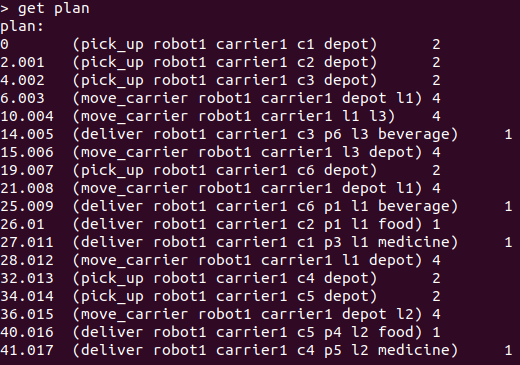
\includegraphics[scale=0.45]{assignment_terminal.png}}
\caption{Plan found by \texttt{POPF} planner.}
\label{fig:plan}
\end{figure}
    
\begin{figure}[t]
\centerline{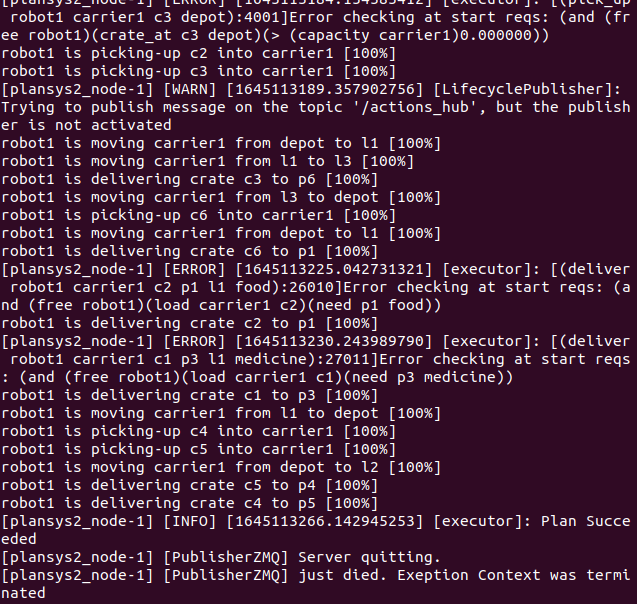
\includegraphics[scale=0.365]{assignment_run.png}}
\caption{\texttt{PlanSys2} execution of the plan.}
\label{fig:execution}
\end{figure}

Executing the \texttt{POPF} planner on this problem, it managed to find the plan shown in Figure 
\ref{fig:plan} of duration 42 seconds.
This plan is then executed by \texttt{PlanSys2} within the \texttt{ROS2} framework. 
Figure \ref{fig:execution} shows part of the execution of the plan and the messages sended by the action nodes.

\section{Conclusions}
\label{sec5}

We have shown how a typical planning problem like the emergency services logistics scenario 
proposed in this report can be solved using the PDDL language and classical planners.

Problems with increasing complexity have been discussed and solved, showing how modern planners can 
efficiently found complex plans.
% This remarks the importance of automated planning for many real applications.

Lastly, we have shown how to integrate the planning problem within the \texttt{PlanSys2} infrastructure
in order to be able to execute the plan in a simulated environment.

In future works, by the use of real robotic agents, it could be interesting to implement real action nodes
and to study the problems that arise in a real environment.

% In future works, it could be interesting use real robotic agents and implement real action nodes in order 
% to solve 



\section{Old}
Planning is the model-based approach to autonomous behavior where the agent behavior is derived
automatically from a model of the actions, sensors, and goals. the main challenges in planning are
computational as all models, whether featuring uncertainty and feedback or not, are intractable in the
worst case when represented in compact form. In this book, we look at a variety of models used in
AI planning, and at the methods that have been developed for solving them. e goal is to provide
a modern and coherent view of planning that is precise, concise, and mostly self-contained, without
being shallow. For this, we make no attempt at covering the whole variety of planning approaches,
ideas, and applications, and focus on the essentials. e target audience of the book are students and
researchers interested in autonomous behavior and planning from an AI, engineering, or cognitive
science perspective.








Nowadays, sport broadcasting plays a large role in current society.
Therefore, it is important to provide a high quality and visually pleasing reporting of sports events.
One common issue in sports is that incidents tend to be over very quickly.
Slow-motion replays can be used to illustrate these incidents as clearly as possible to the viewer. 
Although time is stretched in these replays, there is no exploration of the spatial scene information, which is 
usually important for understanding the event.
A system that allows a replay from any angle adds a lot of value to the viewer experience.

% Especially sports broadcast-
% ing is a well-known recreational aspect of television.
% Therefore, it is important to provide a high quality and
% visually pleasing reporting of sports events.

% In sport most interesting incidents tend to be over very quickly.
% A system that allows a replay from any angle adds a lot of
% value to the production of sport coverage. Sports producers
% may use techniques such as slow-motion replays to illustrate
% these incidents as clearly as possible for the viewer. Although
% time is stretched in these replays, there is no exploration of
% the spatial scene information, which is usually important for
% understanding the event.

Free-viewpoint video (FVV) is one of the recent trends in the development of advanced visual media type
that provides an immersive user experience and interactivity when viewing
visual media. Compared with traditional fixed-viewpoint
video, it allows users to select a viewpoint interactively and
is capable of rendering a new view from a novel viewpoint \cite{05_plane_sweeping}.
Examples of physically impossible camera views which
could be desirable are the goal keepers view, a player tracking camera or even a
ball camera.
% Since a virtualized reality system that distributes 51
% cameras over a 5 m done with controlled lighting and well-calibrated
% cameras was introduced, 
FVV has been a research topic in the field of computer vision 
since a virtualized reality system was developed \cite{04_fast_FVV_01},
ranging from static models for studio applications with a fixed
capture volume, controlled illumination, and backgrounds \cite{02_iview} 
to dynamic object models for sports scenes.
Live outdoor sports such as soccer involve several additional challenges for both acquisition and processing 
phases. 
The action takes place over an entire pitch and video acquisition should be done at sufficient resolution in order to
do analysis and production of desired virtual camera views.

% TODO: si può aggiungere questo...
% Moreover, this has not been confined to academia,
% the companies LiberoVision, Intel, and 4DViews also attach
% importance to the technique and have been providing visual
% effects applications for various purposes.

In this paper, we briefly present and compare the following methods to accomplish free-viewpoint video 
visualization for soccer scenes: the \textit{iview} system \cite{02_iview}, where automatic online camera calibration, 
segmentation and 3D reconstruction is performed,
the work of Goorts et al. \cite{05_plane_sweeping}, where a plane-sweep approach is used,
and the work of Ohta et al. \cite{03_billboard}, where a billboard-based representation is employed to simplify the 
3D model.


% TODO: aggiungere da qualche parte
% There is a demand from the broadcast industry for more flexible production tech-
% nologies at live events such as sports. The ability to place virtual
% cameras at any location around or on the pitch is highly attractive to broadcasters
% greatly increasing flexibility in production and enabling novel delivery formats such
% as mobile TV. Examples of the type of physically impossible camera views which
% could be desirable are the goal keepers view, a player tracking camera or even a
% ball camera.
In the field of computer vision, the techniques for synthesizing virtual view images from a number of real camera
images have been studied since the 1990s.
% Free-viewpoint video in soccer TV broadcast
% production 
% The requirements for free-viewpoint video in sports TV broadcast
% production
Free-viewpoint video in sports TV broadcast production is a challenging problem, involving the conflicting requirements of 
broadcast picture quality with video-rate generation.
FVV techniques for generating novel viewpoints using a multiview camera setup can be categorized into two classes 
\cite{05_plane_sweeping}: 3D reconstruction and image-based rendering. 

Using 3D reconstruction, it is possible to construct 3D models of objects that provides a geometric proxy, which can be
used to combine observations from multiple views in order to render images from an arbitrary viewpoint. 
Several approaches have been realized for reconstruction: visual-hull, photo-hull, stereo and 
global shape optimisation \cite{02_iview}.
% TODO: si può scrivere di più da 02
The quality of the virtual view image generated
by these methods depends on the accuracy of the 3D model. In order to produce an accurate model, a
large number of video cameras surrounding the object should be used. 
Although 3D reconstruction is robust, artifacts such as ghosting objects can be introduced if a lot of objects are in the scene. 

Image-based methods generate the image of the novel viewpoint directly without explicitly reconstructing the 3D scene structure.
The quality of rendered views depends on the accuracy of alignment between multiple view observations 
\cite{05_plane_sweeping,02_iview}.
Usually, these methods are limited to rendering viewpoints between the camera views.
% In many
% methods, depth generation, implicit or explicit, is
% done concurrently.



% Moreover, ... TODO:01
% Furthermore,
% camera calibration [13] is usually required to relate 2-D co-
% ordinates in images to their corresponding 3-D coordinates in
% object space. As it is essential to measure the 3-D positions of
% several points in the object space, calibration becomes difficult
% especially in a large space. For these reasons, the object area is
% generally limited to a few cubic meters in this approach.

% TODO: overview dei sistemi esistenti presente in 02

\section{Design Choices}
In this section, we present the DTI-funded collaborative project \textit{iview} \cite{iview_project},
a free-viewpoint video system which enables the production of novel desirable camera views.
This system exploits the already placed live TV broadcast cameras as the primary
source of multiple view video.
Usually, soccer matches are covered by 12-20 high-definition cameras placed all over in the stadium
providing wide-baseline views.
Match cameras are manually controlled to follow the game play zooming in on events.
However, only a fraction of these are focused on specific events of interest and can be used for production 
of free-viewpoint renders, the remaining cameras cover the pitch, crowd and coaches.


% Robust algorithms are required for both recovery of camera
% calibration from the broadcast footage and wide-baseline correspondence between
% views for reconstruction or view interpolation.

% Therefore
% iview uses a method for real-time camera calibration from the match footage [2:46].
% Player segmentation is performed using chroma-key and difference matting tech-
% niques independently for each camera view [2:15]. Automatic calibration and player
% segmentation for moving broadcast cameras results in errors of the order of 1-3
% pixels which is often comparable to the size of players arms and legs in the broad-
% cast footage. Robust reconstruction and rendering of novel viewpoints is achieved in
% the iview system by an initial conservative visual-hull reconstruction followed by a
% view-dependent refinement. View-dependent refinement simultaneously refines the
% player reconstruction and segmentation exploiting visual cues from multiple cam-
% era views. This achieves free-viewpoint rendering with pixel accurate alignment of
% neighbouring views to render novel views with a visual quality approaching that
% of the source video.

% Advances are presented in real-time through the
% lens camera calibration to estimate both the camera pose, focus and lens distortion
% from the pitch marks.

% Free-viewpoint video is then produced starting with a volu-
% metric reconstruction followed by a view-dependent refinement using information
% from multiple views.

% Automatic online calibration, segmentation and reconstruction is performed to allow
% rendering of novel viewpoints from the moving match cameras.

\begin{figure}[htbp]
\centerline{\includegraphics[scale=0.078]{iview_overview2.png}}
\caption{Overview of the \textit{iview} free-viewpoint video system \cite{02_iview}.}
\label{fig:iview_overview}
\end{figure}


The \textit{iview} system is composed of three main modules as shown in Figure \ref{fig:iview_overview}: 
capture, processing and replay module.

Capture is performed using time synchronised acquisition from both auxiliary and
match cameras.
The minimal number of cameras is about four, but for good quality results a higher number is required.
Camera synchronisation is achieved using standard genlock process.

The processing module computes a 3D model of the scene.
This is done using segmentation of objects from the background and 3D reconstruction \cite{2.1_iview}.

To allow the use of footage from match cameras and to avoid the need for prior calibration, 
automatic calibration of all cameras is performed using a line-based approach against the pitch lines of the captured footage, 
achieving a root-mean-square error of 1-2 pixels for moving cameras. 
The calibration is very fast and robust, capable of real-time operation for use during live match footage. 
Calibration estimates the extrinsic and intrinsic parameters of each camera including lens distortion.

The segmentation is needed to separate the foreground, i.e., the players, from the background.
Matting of players from the green pitch is performed using chroma-keying matting. 
% This allows the approximate segmentation of the foreground players for subsequent processing to produce free-viewpoint video. 
The authors developed and tested a k-nearest neighbour approach for chroma-keying and evaluated two other known techniques,
\textit{Fast green subtraction} in RGB colour space and keying in HSV colour space.
The k-nearest neighbour classifier is controlled by a GUI where the user has to click on position in the image that corresponds
to the background. 
The process is repeated until the resulting segmentation is satisfying.
A deeper explanation is present in the paper \cite{2.1_iview} where the authors present and evaluate also 
\textit{Fast green subtraction} and keying in HSV.

The accumulation of errors from calibration and matting can cause large errors in
the reconstruction of the scene, such as loss of limbs. 
Therefore, robust algorithms have been developed for scene reconstruction.
One possible technique is called visual-hull (VH) and represents the maximum volume occupied by an object
given a set of silhouettes from multiple views \cite{2.2_iview_08}.
The visual-hull is a single global representation integrating silhouette information from all
views. A polygonal mesh surface is typically extracted and texture mapped by resampling
the captured multiple view video for rendering \cite{2.2_iview}.
Due to accumulating errors in camera calibration and segmentation, visual-hull accuracy is reduced.
A refinement of the view-dependent visual hull (VDVH) \cite{2.1_iview_12},
using stereo correspondence to interpolate between captured
views, can be used to overcome these issues, achieving the best alignment between adjacent views and 
hence improving visual quality.
More information about \textit{iview} 3D reconstruction can be found in \cite{02_iview,2.1_iview,2.2_iview}.

Finally, the replay module renders the novel view of the scene using the computed 3D model together with the
original camera images.
Cameras closer to the virtual viewpoint are chosen to generate the novel viewpoint.
% TODO: può essere descritto maggiormente the replay module 


The method proposed achieves an image quality comparable to that of the input images and it is robust to the
wide-baseline moving camera views at different resolutions.
Calibration and segmentation are very important in order to obtain an overall good quality of the system.
Degradation in image quality will also occur if there are insufficient views for reconstruction.
% TODO: si può aggiungere contenuto

% Aperture correction is also applied to each video sequence to correct for the camera edge enhancement
% used in standard broadcast footage \cite{iview}.

% Likewise matting in relatively uncontrolled outdoor conditions with changing illu-
% mination achieves a segmentation within 1-2 pixels of the true foreground with the
% addition of background clutter for the crowd, hoardings and on-pitch advertising.





% The replay module renders the captured scene in realtime
% using the computed 3D model and the original camera images
% deploying view-dependent texture mapping [8].
% The entire system can potentially operate in real-time. At
% the current stage the processing is done offline. That means
% the images are stored and the processing is run at a later stage.
% The replay module is designed to work at interactive rates.
\section{Image-based rendering - extended plane sweeping}

% \begin{figure*}[htbp]
% \centerline{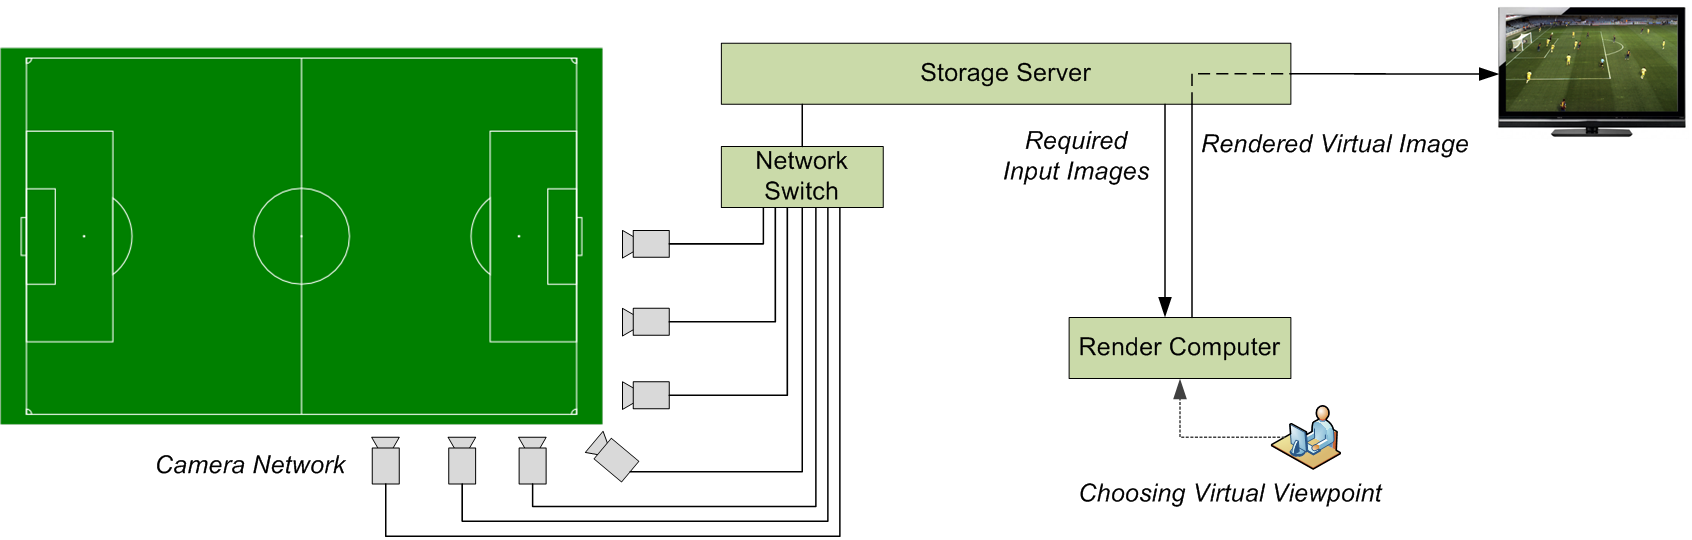
\includegraphics[scale=0.18]{plane_sweeping.png}}
% \caption{}
% \label{fig:plane_sweeping}
% \end{figure*}

\begin{figure*}[htbp]
\centerline{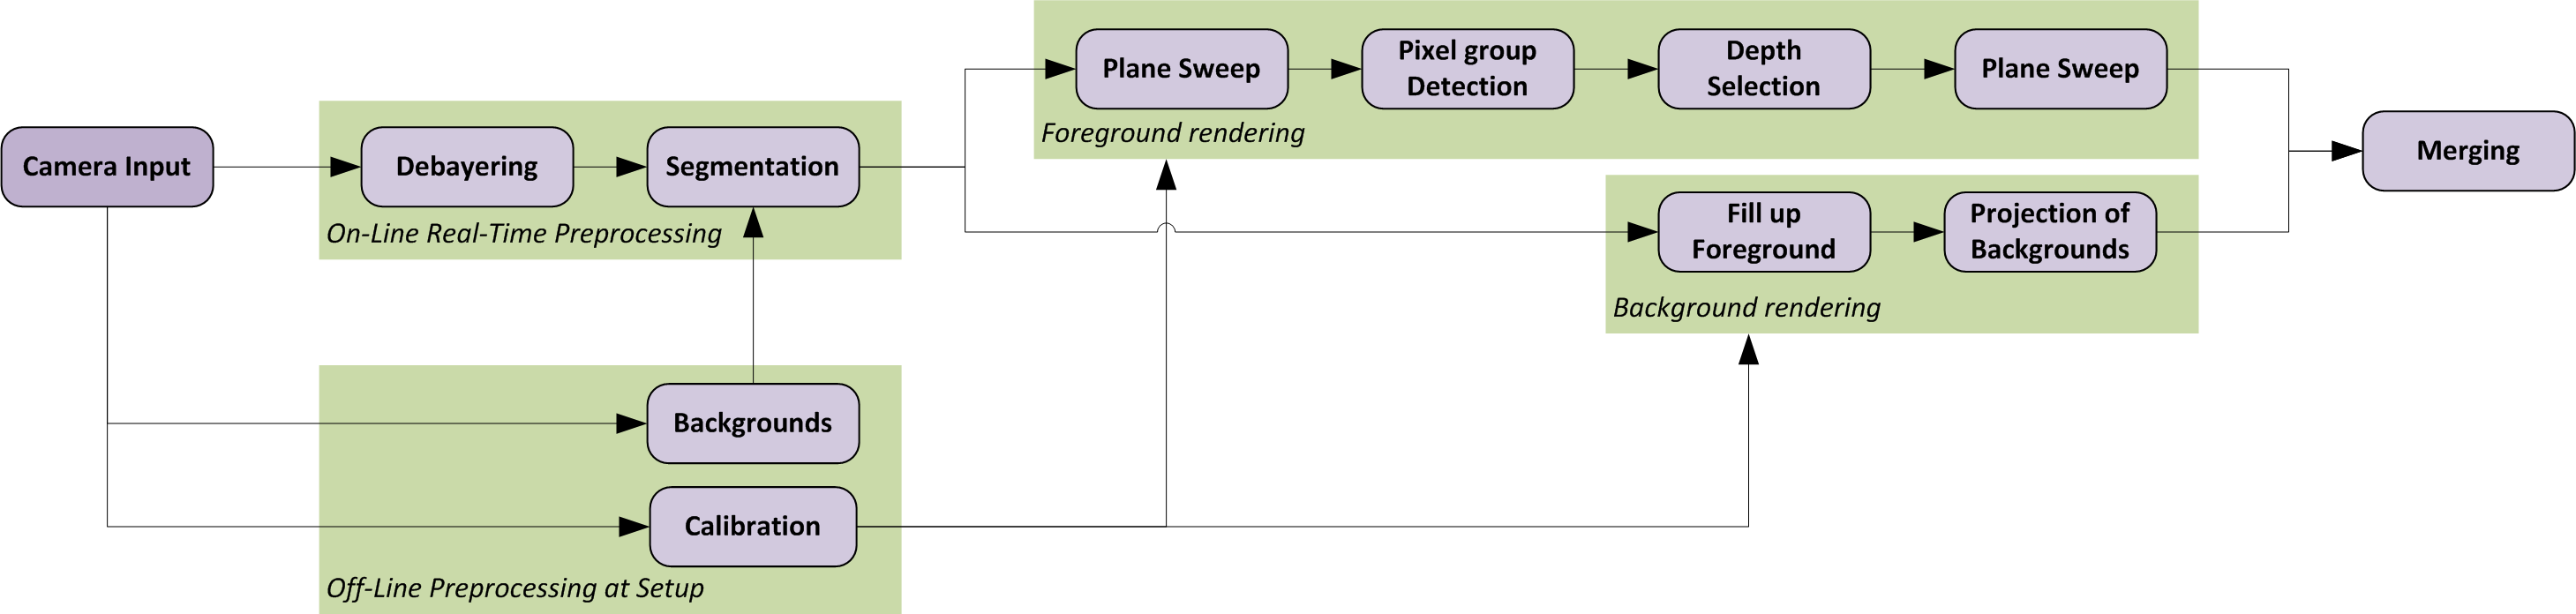
\includegraphics[scale=0.18]{plane_sweeping2.png}}
\caption{Overview of the extended plane sweeping method. Both the non real-time and real-time phase are shown \cite{05_plane_sweeping}.}
\label{fig:plane_sweeping2}
\end{figure*}

In this section, we present the work of Goorts et al. \cite{05_plane_sweeping}, i.e., an image-based approach to generate 
virtual camera view interpolating real camera images.
Instead of performing 3D reconstruction, image-based methods directly generate the image of the novel viewpoint.
When multiple cameras are present, plane sweeping can be used \cite{05_plane_sweeping_yang} for both small and wide 
baseline setups.
Plane sweeping has already been used for novel viewpoint in soccer scenes. Goorts et al. \cite{05_plane_sweeping_2013} 
present a method with two plane sweeps and a depth filtering step suitable for smaller baseline 
setups of about 1 meter. 
This method presents some problems like disappearing players
when they overlap in the image.

The method presented here is fully automatic and employs GPU
parallel processing to achieve fast processing speed.
The system setup consists of 7 static cameras placed in a
wide baseline setup, i.e., 10 meters between each camera.
All cameras are synchronized on shutter level using a global clock.
% All images are transferred to a storage server,
% where all the captured data is stored. A render com-
% puter can access all required images to generate a
% novel viewpoint.
The generation of novel viewpoint consists of two steps as shown in Figure \ref{fig:plane_sweeping2}:
a first off-line preprocessing phase and a real-time interpolation phase. 

The preprocessing phase is responsible for camera calibration and background determination.
Cameras are calibrated in order to acquire their position, orientation and extrinsic and intrinsic parameters.
The calibration method of Svoboda et al. \cite{05_plane_sweeping_Svoboda} has been employed for this purpose:
SIFT features are extracted from a number of frames and the pairwise matching between them is calculated 
using the k-d tree algorithm; these matches are tracked across different image pairs obtaining point 
correspondences between multiple images \cite{05_plane_sweeping}.
The background of every image stream is determined using a per-pixel median approach applied to about 30 images
per stream (2 seconds apart each other).


The real-time phase generates images for a chosen virtual camera position and a chosen time in the video sequence.
First, camera images are debayered and segmented. These images are then used to process foreground and background independently.
The foreground rendering uses a plane-sweep approach followed by depth filtering and a depth-selective plane sweep 
as explained in \cite{05_plane_sweeping}.
The foreground and background are then merged together according to the segmentation information.

Debayering consists of converting the raw images to its RGB representation.
Segmentation is based on backgrounds obtained during off-line preprocessing and is performed on a per-pixel basis using
the differences between the color values and three thresholds.
This allows fast segmentation in high quality.


Applying this method, the authors obtained high quality results using wide baseline setup and typical artifacts of normal plane sweeping, 
such as ghost players, are removed.
Some other artifacts can still be present, such as ghost lines, caused by the simplified assumption of the geometry of the pitch.
% , where the
% reprojection consistency for different depths is maxi-
% mized, thus generating a novel image and depth map
% simultaneously. However, normal plane sweeping
% does not yield high quality results for soccer scenes
% using a wide baseline setup. Serious artifacts, such as
% ghost players, can be perceived. Therefore, we em-
% ploy a depth selection method where the acceptable
% depths of groups of pixels is determined and used in a
% second, depth-selective plane sweep.
% To demonstrate our method, we obtained images
% from a real soccer match in real conditions. Our
% method outperforms other free viewpoint video sys-
% tems, as demonstrated by the results and the accompa-
% nying video. Typical artifacts, such as ghost players,
% are effectively removed.
\section{Billboard-based visualization}
In this section, we present the work of Ohta et al. \cite{03_billboard}.
The authors use billboard representation to make a 3D model of each player.
This method is simpler than full 3D reconstruction and requires less computation.
A player billboard is a small rectangle standing perpendicular to the ground
and a 2D texture is shown on it.
The difference between 3D reconstruction and billboard representation is shown in Figure \ref{fig:billboard_comparison}:
as we can see, the visual difference is clear at a close viewpoint but becomes very small at a distant one.
For this reason, becomes particularly important to place player billboards at a right place and direction.

\begin{figure}[htbp]
\centerline{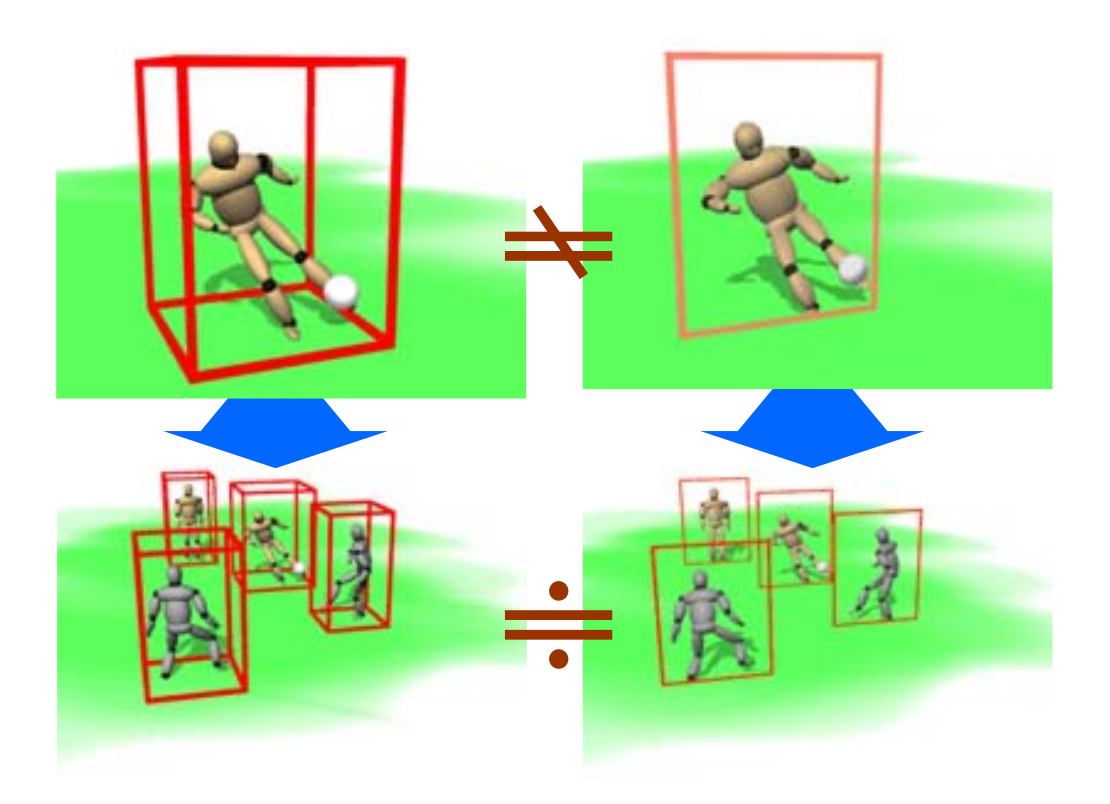
\includegraphics[scale=0.22]{billboard_comparison.png}}
\caption{Appearance similarity between 3D reconstruction and billboard in close and distant view \cite{03_billboard}.}
\label{fig:billboard_comparison}
\end{figure}


The system proceeds as follows: first it extracts texture segments from camera videos, then selects appropriate textures according
to the virtual viewpoint and finally layouts the player billboards in virtual space.

Texture extraction phase consists in obtaining the location of each player and extracting texture segments from every image 
video by projecting player location onto the image plane.
Background region is removed in the texture by video capturing PC.
Please note that camera calibration is done before this phase.

Texture selection phase selects a set of texture to be sent to each viewer based on his viewpoint. 
Given a viewpoint, the system finds the camera that minimizes the angle between the line from the viewpoint to the player 
location and the line from the camera to the player location. Then, a texture segment obtained by that camera is selected 
and placed so that the texture faces the viewpoint \cite{03_billboard}.
% TODO: completare


One problem may happen when players are overlapped each other at a certain camera and billboard texture might include both
of them.
To eliminate extra player region, authors used stereo based method \cite{03_billboard_04} as explained in \cite{03_billboard}. 
% TODO: can be explained more



\section{Conclusion}
We have briefly presented three free-viewpoint systems for soccer games: the \textit{iview} system, an image-based method using 
plane sweeping and a billboard-based method.

The \textit{iview} system is a robust method using a multi-camera setup that performs 3D reconstruction exploiting a refinement 
of the view-dependent visual hull method.
% This method requires % TODO: finire

The image-based method presented interpolates real camera images using a plane sweeping approach.
High quality images using wide baseline setup are obtained and typical artifacts are removed.

The billboard-based method is simpler than full 3D reconstruction and requires less computation.
However, this method produces lower quality images and some visual artifacts can be present.





\bibliographystyle{IEEEtran}
\bibliography{biblio.bib}



\end{document}